% begin module IVT
\begin{frame}
\begin{theorem}[The Intermediate Value Theorem]
Suppose $f$ is continuous on the closed interval $[a,b]$ and \alertNoH{2,4,6,8}{let $N$ be any number between $f(a)$ and $f(b)$}, where $f(a) \neq f(b)$.  Then there \alertNoH{3,5,7,9}{exists a number $c$} in $(a,b)$ \alertNoH{3,5,7,9}{such that $f(c) = N$}.
\end{theorem}
\begin{center}

\begin{pspicture}(-1.5,-0.5)(6.2,4)
\psframe*[linecolor=white](-0.5,-0.5)(6.2,4) 
\psaxes[labels=none, ticks=none]{<->}(0,0)(-0.5, -0.5)(6.2,4)
\psplot[linecolor=red, plotpoints=1000]{1}{6}{x 4.42857 mul x x mul -1.42857 mul add x x mul x mul 0.142857 mul add -2.42857 add }

\psline[linestyle=dashed](1,0.714285714)(1,0)
\psline[linestyle=dashed](0,0.714285714)(1, 0.714285714)
\rput[t](1, -0.1){$a$}
\rput[r](-0.1,0.714285714){$f(a)$}

\psline[linestyle=dashed](6,3.571428571)(6,0)
\psline[linestyle=dashed](0,3.571428571)(6, 3.571428571)
\rput[t](6, -0.1){$b$}
\rput[r](-0.1,3.571428571){$f(b)$}


\only<handout:0|2-3>{
\rput[r](-0.1,3.073142857){\alert<2>{$N$}}
\psline(-0.05, 3.073142857)(0.05,3.073142857)
}
\only<handout:0|3>{
\psline[linecolor=blue, linestyle=dashed](5.8,3.073142857)(5.8,0)
\psline[linecolor=blue, linestyle=dashed](0,3.073142857)(5.8, 3.073142857)
\rput[t](5.8, -0.1){\alert<3>{$c$}}
}
\only<handout:0|4-5>{
\rput[r](-0.1,2.482142857){\alert<4>{$N$}}
\psline(-0.05, 2.482142857)(0.05,2.482142857)
}
\only<handout:0|5>{
\psline[linecolor=blue, linestyle=dashed](5.5,2.482142857)(5.5,0)
\psline[linecolor=blue, linestyle=dashed](0,2.482142857)(5.5, 2.482142857)
\rput[t](5.5, -0.1){\alert<5>{$c$}}
}
\only<handout:0|6-7>{
\rput[r](-0.1,2.182428571){\alert<6>{$N$}}
\psline(-0.05, 2.182428571)(0.05,2.182428571)
} %
\only<handout:0|7>{
\psline[linecolor=blue, linestyle=dashed](5.3,2.182428571)(5.3,0)
\psline[linecolor=blue, linestyle=dashed](0,2.182428571)(5.3, 2.182428571)
\rput[t](5.3, -0.1){\alert<7>{$c$}}
} %

\only<handout:0|8-9>{
\rput[r](-0.1,1.857142857){\alert<8>{$N$}}
\psline(-0.05, 1.857142857)(0.05,1.857142857)
}
\only<9>{
\psline[linecolor=blue, linestyle=dashed](0,1.857142857)(5,1.857142857)
\psline[linecolor=blue, linestyle=dashed](3,1.857142857)(3, 0)
\psline[linecolor=blue, linestyle=dashed](5,1.857142857)(5, 0)
\psline[linecolor=blue, linestyle=dashed](2,1.857142857)(2, 0)
\rput[t](2, -0.1){\alertNoH{9}{$c_1$}}
\rput[t](3, -0.1){\alertNoH{9}{$c_2$}}
\rput[t](5, -0.1){\alertNoH{9}{$c_3$}}
}
\end{pspicture}
%\ \only<handout:0| -1>{%
%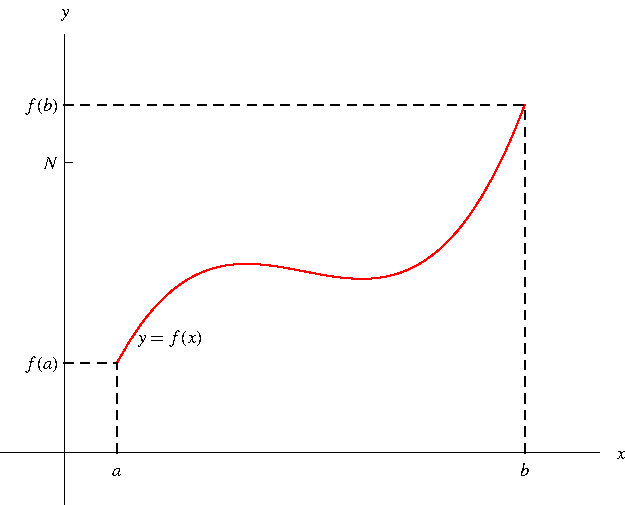
\includegraphics[height=6cm]{continuity/pictures/02-05-ivta.pdf}%
%}%
%\only<handout:0| 2>{%
%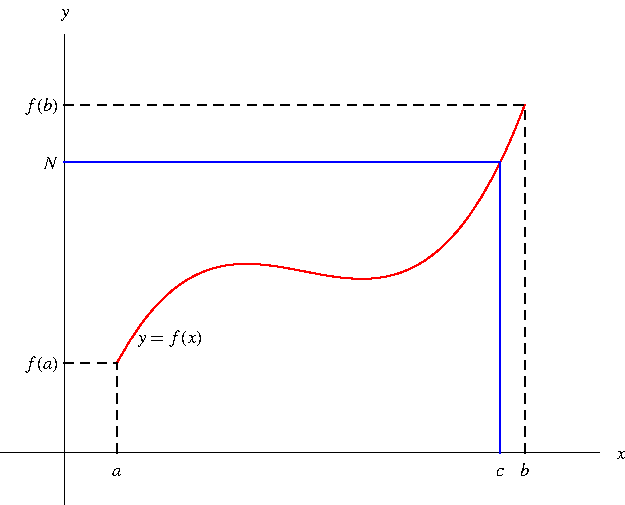
\includegraphics[height=6cm]{continuity/pictures/02-05-ivtb.pdf}%
%}%
%\only<handout:0| 3>{%
%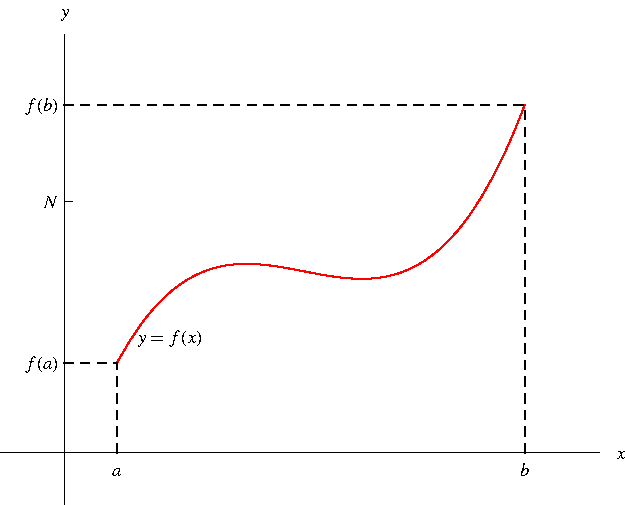
\includegraphics[height=6cm]{continuity/pictures/02-05-ivtc.pdf}%
%}%
%\only<handout:0| 4>{%
%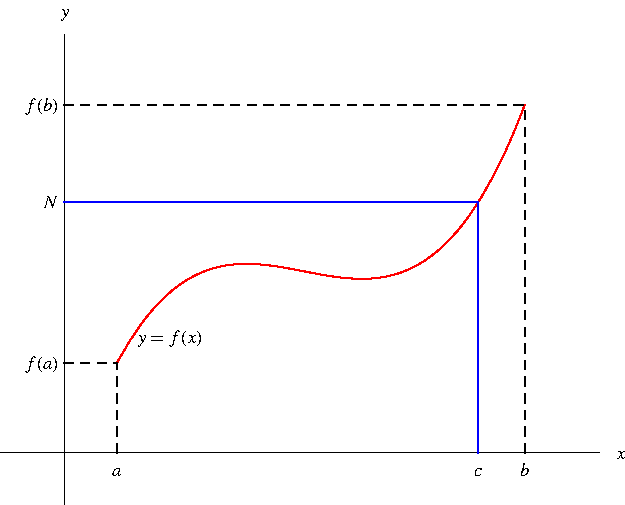
\includegraphics[height=6cm]{continuity/pictures/02-05-ivtd.pdf}%
%}%
%\only<handout:0| 5>{%
%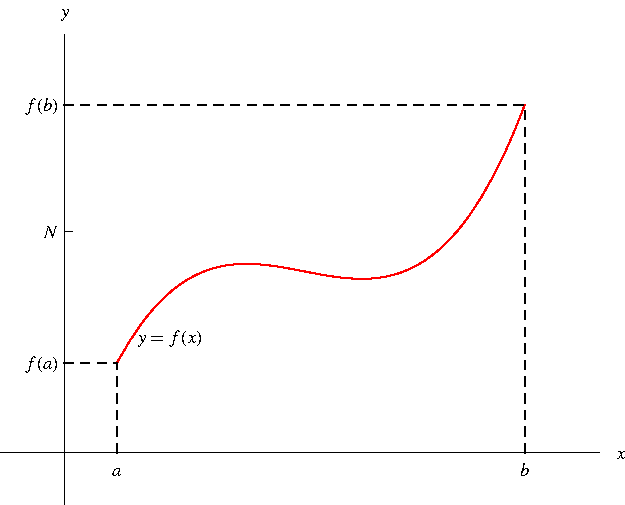
\includegraphics[height=6cm]{continuity/pictures/02-05-ivte.pdf}%
%}%
%\only<6>{%
%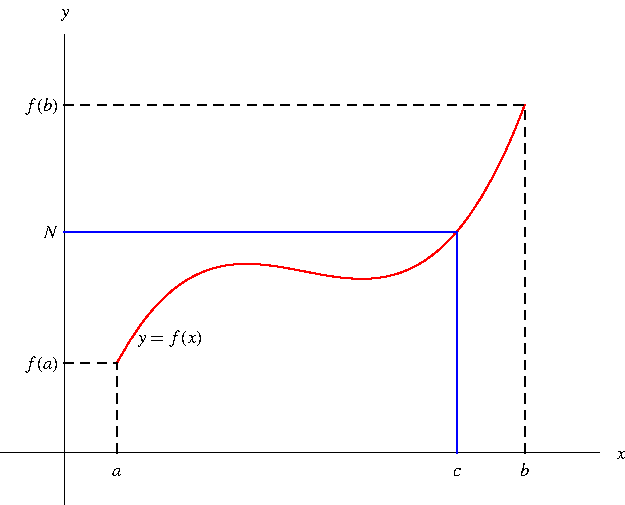
\includegraphics[height=6cm]{continuity/pictures/02-05-ivtf.pdf}%
%}%
%\only<handout:0| 7>{%
%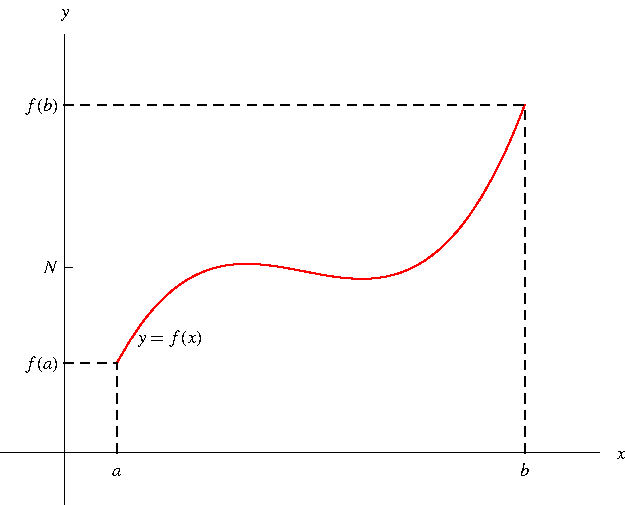
\includegraphics[height=6cm]{continuity/pictures/02-05-ivtg.pdf}%
%}%
%\only<handout:0| 8->{%
%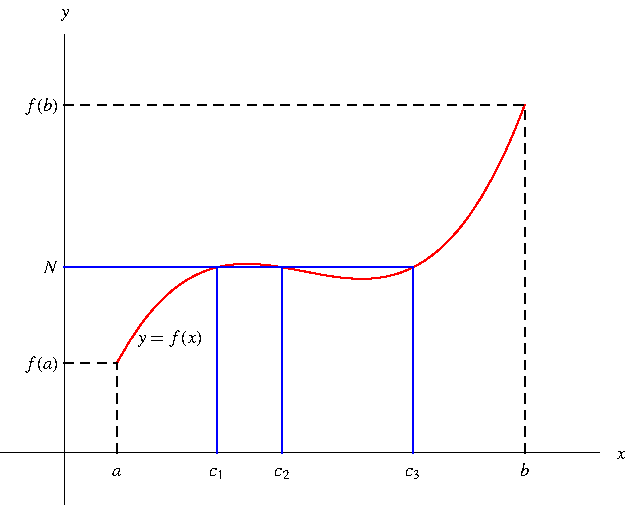
\includegraphics[height=6cm]{continuity/pictures/02-05-ivth.pdf}%
%}%
\end{center}
\end{frame}
% end module IVT
